\subsection{Resumo}

\begin{table}[h!]
\centering
\begin{tabular}{ |c|c|c|c|c|  }
\hline
\rowcolor{lightgray}
Algoritmo & Max & Min & Média & Desvio Padrão \\
\hline
Hill-Climbing & 1.382 & 0.163 & 0.871 & 0.448 \\
\hline
Hill-Climbing com restart & 1.864 & 0.0 & 0.777 & 0.645 \\
\hline
Simulated Annealing & 1.915 & 0.774 & 1.317 & 0.435 \\
\hline
Genetic Algorithm & 1.148 & 0.003 & 0.263 & 0.361 \\
\hline

\end{tabular}
\caption{Tabela com dados consolidados dos algoritmos}
\end{table}

\begin{figure}[H]
\centering
  \begin{minipage}[b]{0.48\textwidth}
    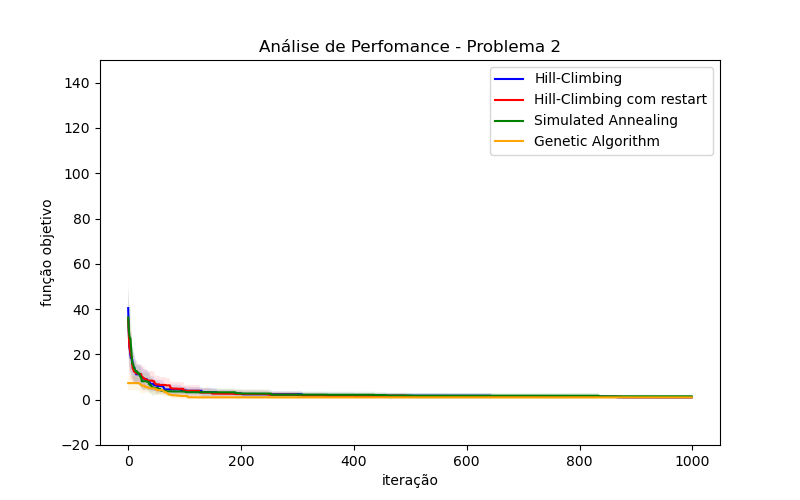
\includegraphics[width=88mm]{imagens/otima/problema-2-performance-algoritmos-best.png}
    \caption{Dados da execução da função objetivo durante as 10 iterações por melhor valor.
    \label{fig:problema-2-performance-algoritmos-best}}
  \end{minipage}
  \hfill
  \begin{minipage}[b]{0.48\textwidth}
    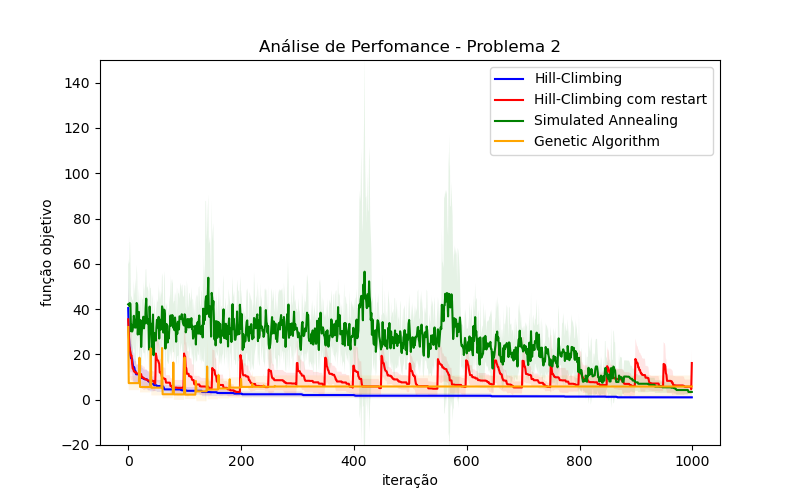
\includegraphics[width=88mm]{imagens/otima/problema-2-performance-algoritmos-value.png}
    \caption{Dados da execução da função objetivo durante as 10 iterações por valor atual.
    \label{fig:problema-2-performance-algoritmos-value}}
  \end{minipage}
\end{figure}